\documentclass[12pt]{article}
\usepackage[english]{babel}
\usepackage[utf8]{inputenc}
\usepackage{amsmath, amssymb, amsthm}
\usepackage{graphicx}
\usepackage{hyperref}
\usepackage{geometry}
\usepackage{xcolor}
\usepackage{tikz}

\setlength{\topmargin}{0pt}
\setlength{\headsep}{0pt}
\textheight = 600pt

\title{Graph Theory \\ Homework 2}
\author{Ben Kallus and Maddy LaPoint}
\date{Due Wednesday, February 10}

\begin{document}
\pagecolor{black}
\color{white}
\maketitle

\noindent{\bf 1.16}

\noindent{\bf Proposition:} Let $P = (u=v_0,v_1,...,v_k=v)$, $k\geq 1$, be a $u - v$ geodesic in a connected graph $G$. Then, $d(u,v_i) = i$ for each integer $i$ with $1 \leq i \leq k$.
\begin{proof}
    Let $P = (u = v_0, v_1, \hdots, v_k = v)$, $k \geq 1$, be a $u-v$ geodesic in a connected graph $G$.
    Since $P$ has length $k$, $d(u,v)=k$.
    Suppose, toward a contradiction, that there exists an integer $i$ such that $1 \leq i \leq k$ and $d(u,v_i) \neq i$.
    Then $d(u,v_i) < i$, since $(u = v_0, \hdots, v_i)$ is a $u-v_i$ walk of length $i$.
    Therefore, there exists a $u-v_i$ path $Q = (u=q_0, q_1, \hdots, q_j=v_i)$ with length $j < i$.
    Define $R$ to be $(u=q_0, q_1, \hdots, q_j=v_i, v_{i+1}, \hdots, v_k)$.
    The length of $R$ is therefore $k - i + j$.
    Thus, since $j$ is less than $i$, the length of $R$ is less than $k$.
    Thus, $d(u,v) < k$. Since $d(u,v) = k$, this is a contradiction.
    Thus, $d(u,v_i)=i$ for each integer $i$ with $1 \leq i \leq k$.
\end{proof}

\bigskip
\noindent{\bf 1.15}
\begin{center}
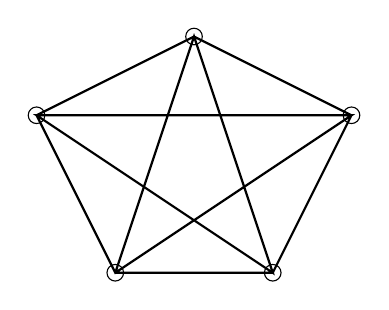
\begin{tikzpicture}
    \draw[fill=white] (1,0) circle (3pt);
    \draw[fill=white] (3,0) circle (3pt);
    \draw[fill=white] (4,2) circle (3pt);
    \draw[fill=white] (2,3) circle (3pt);
    \draw[fill=white] (0,2) circle (3pt);

    \draw[thick] (1,0) -- (3,0) -- (4,2) -- (2,3) -- (0,2) -- (1,0) -- (4,2) -- (0,2) -- (3,0) -- (2,3) -- (1,0);
\end{tikzpicture}
\end{center}

    % Should this be more formal?
    Suppose there were another graph $G$ of order 5 with odd distances between every two distinct vertices.
    Then, since $G$ is not $K_5$, there exist two vertices $u,v \in V(G)$ with $d(u,v) \geq 3$.
    Thus, there exists a $u-v$ geodesic $P = (u=v_0, v_1, \hdots, v_{d(u,v)}=v)$ with length at least 3.
    By the result of exercise 1.16, $d(u,v_2) = 2$.
    Thus, $K_5$ is the only graph of order 5 with odd distances between every two distinct vertices.

\newpage
\noindent{\bf 1.17}

\noindent{\bf (a) Proposition:} Let $P$ and $Q$ be two longest paths in a connected graph. Then $P$ and $Q$ have at least one vertex in common.
\begin{proof}
    Let $G$ be a connected graph.
    Let $P=(p_0, p_1,\hdots,p_k)$ and $Q=(q_0, q_1,\hdots, q_k)$ be two longest paths in $G$.
    Suppose, toward a contradiction, that $P$ and $Q$ have no vertex in common.
    Then, since $G$ is connected, there exists at least one nontrivial path that begins at a vertex in $P$ and terminates at a vertex in $Q$.
    Define $M$ to be the set of lengths of all such paths.
    Since $M \subseteq \mathbb N$, $M$ has a minimal element, $m$, by the well-ordering principle.
    Thus, there exists a path $R$ of length $m$ that begins at a vertex $p_i \in P$ and terminates at a vertex $q_j \in Q$, for some $i,j$ satisfying $0 \leq i,j \leq k$.
    Note that the only vertex shared between $R$ and $P$ is $p_i$, since the presence of another such vertex would indicate that $R$ is not a minimum-length path beginning at a vertex in $P$ and ending at a vertex in $Q$.
    By a symmetric argument, the only vertex shared between $R$ and $Q$ is $q_j$.
    Define $P'$ to be the longest of the two paths $(p_0, p_1, \hdots, p_i)$ and $(p_k, p_{k-1}, \hdots, p_i)$. % What if they're the same length?
    Define $Q'$ to be the longest of the two paths $(q_j, q_{j-1}, \hdots, q_0)$ and $(q_j, q_{j+1}, \hdots, q_k)$.
    Note that this definition ensures that the lengths of $P'$ and $Q'$ are at least $\frac k2$.
    Define $X$ to be the concatenation of $P'$, $R$, and $Q'$.
   Then, $X$ is a path, since $P'$ shares no vertices with $Q'$, and $R$ shares no vertices with $P'$ and $Q'$, other than its first and last.
    Then, the length of $X$ is at least $\frac k2 + 1 + \frac k2 = k + 1$.
    Since the longest path in $G$ has length $k$, this is a contradiction.
    Thus, $P$ and $Q$ have a vertex in common.
\end{proof}
\medskip
\noindent{\bf (b) Counterexample:}
    Let $G$ be the complete graph of order 4, with vertices $\{c_1, c_2, c_3, c_4\}$.
    Since there exists an edge between all pairs of distinct vertices in $G$, it has diameter 1.
    Observe that the edges $c_1c_2$ and $c_3c_4$ are geodesics of length 1 that do not share a vertex.
    Thus, two geodesics of maximal length in $G$ do not necessarily have a vertex in common.

\bigskip
\noindent{\bf 1.19}
This statement is not true.
Let $G$ be the path graph of order 4, with vertices $\{p_0, p_1, p_2, p_3\}$, and edges $\{p_0p_1, p_1p_2, p_2p_3\}$.
Clearly, $G - p_1$ and $G - p_2$ are disconnected.
Thus, since $G$ has only 4 vertices, there do not exist three vertices $u,v,w \in V(G)$ such that $G-u,G-v,G-w$ are all connected.

\bigskip
\noindent{\bf 1.21}
\begin{center}
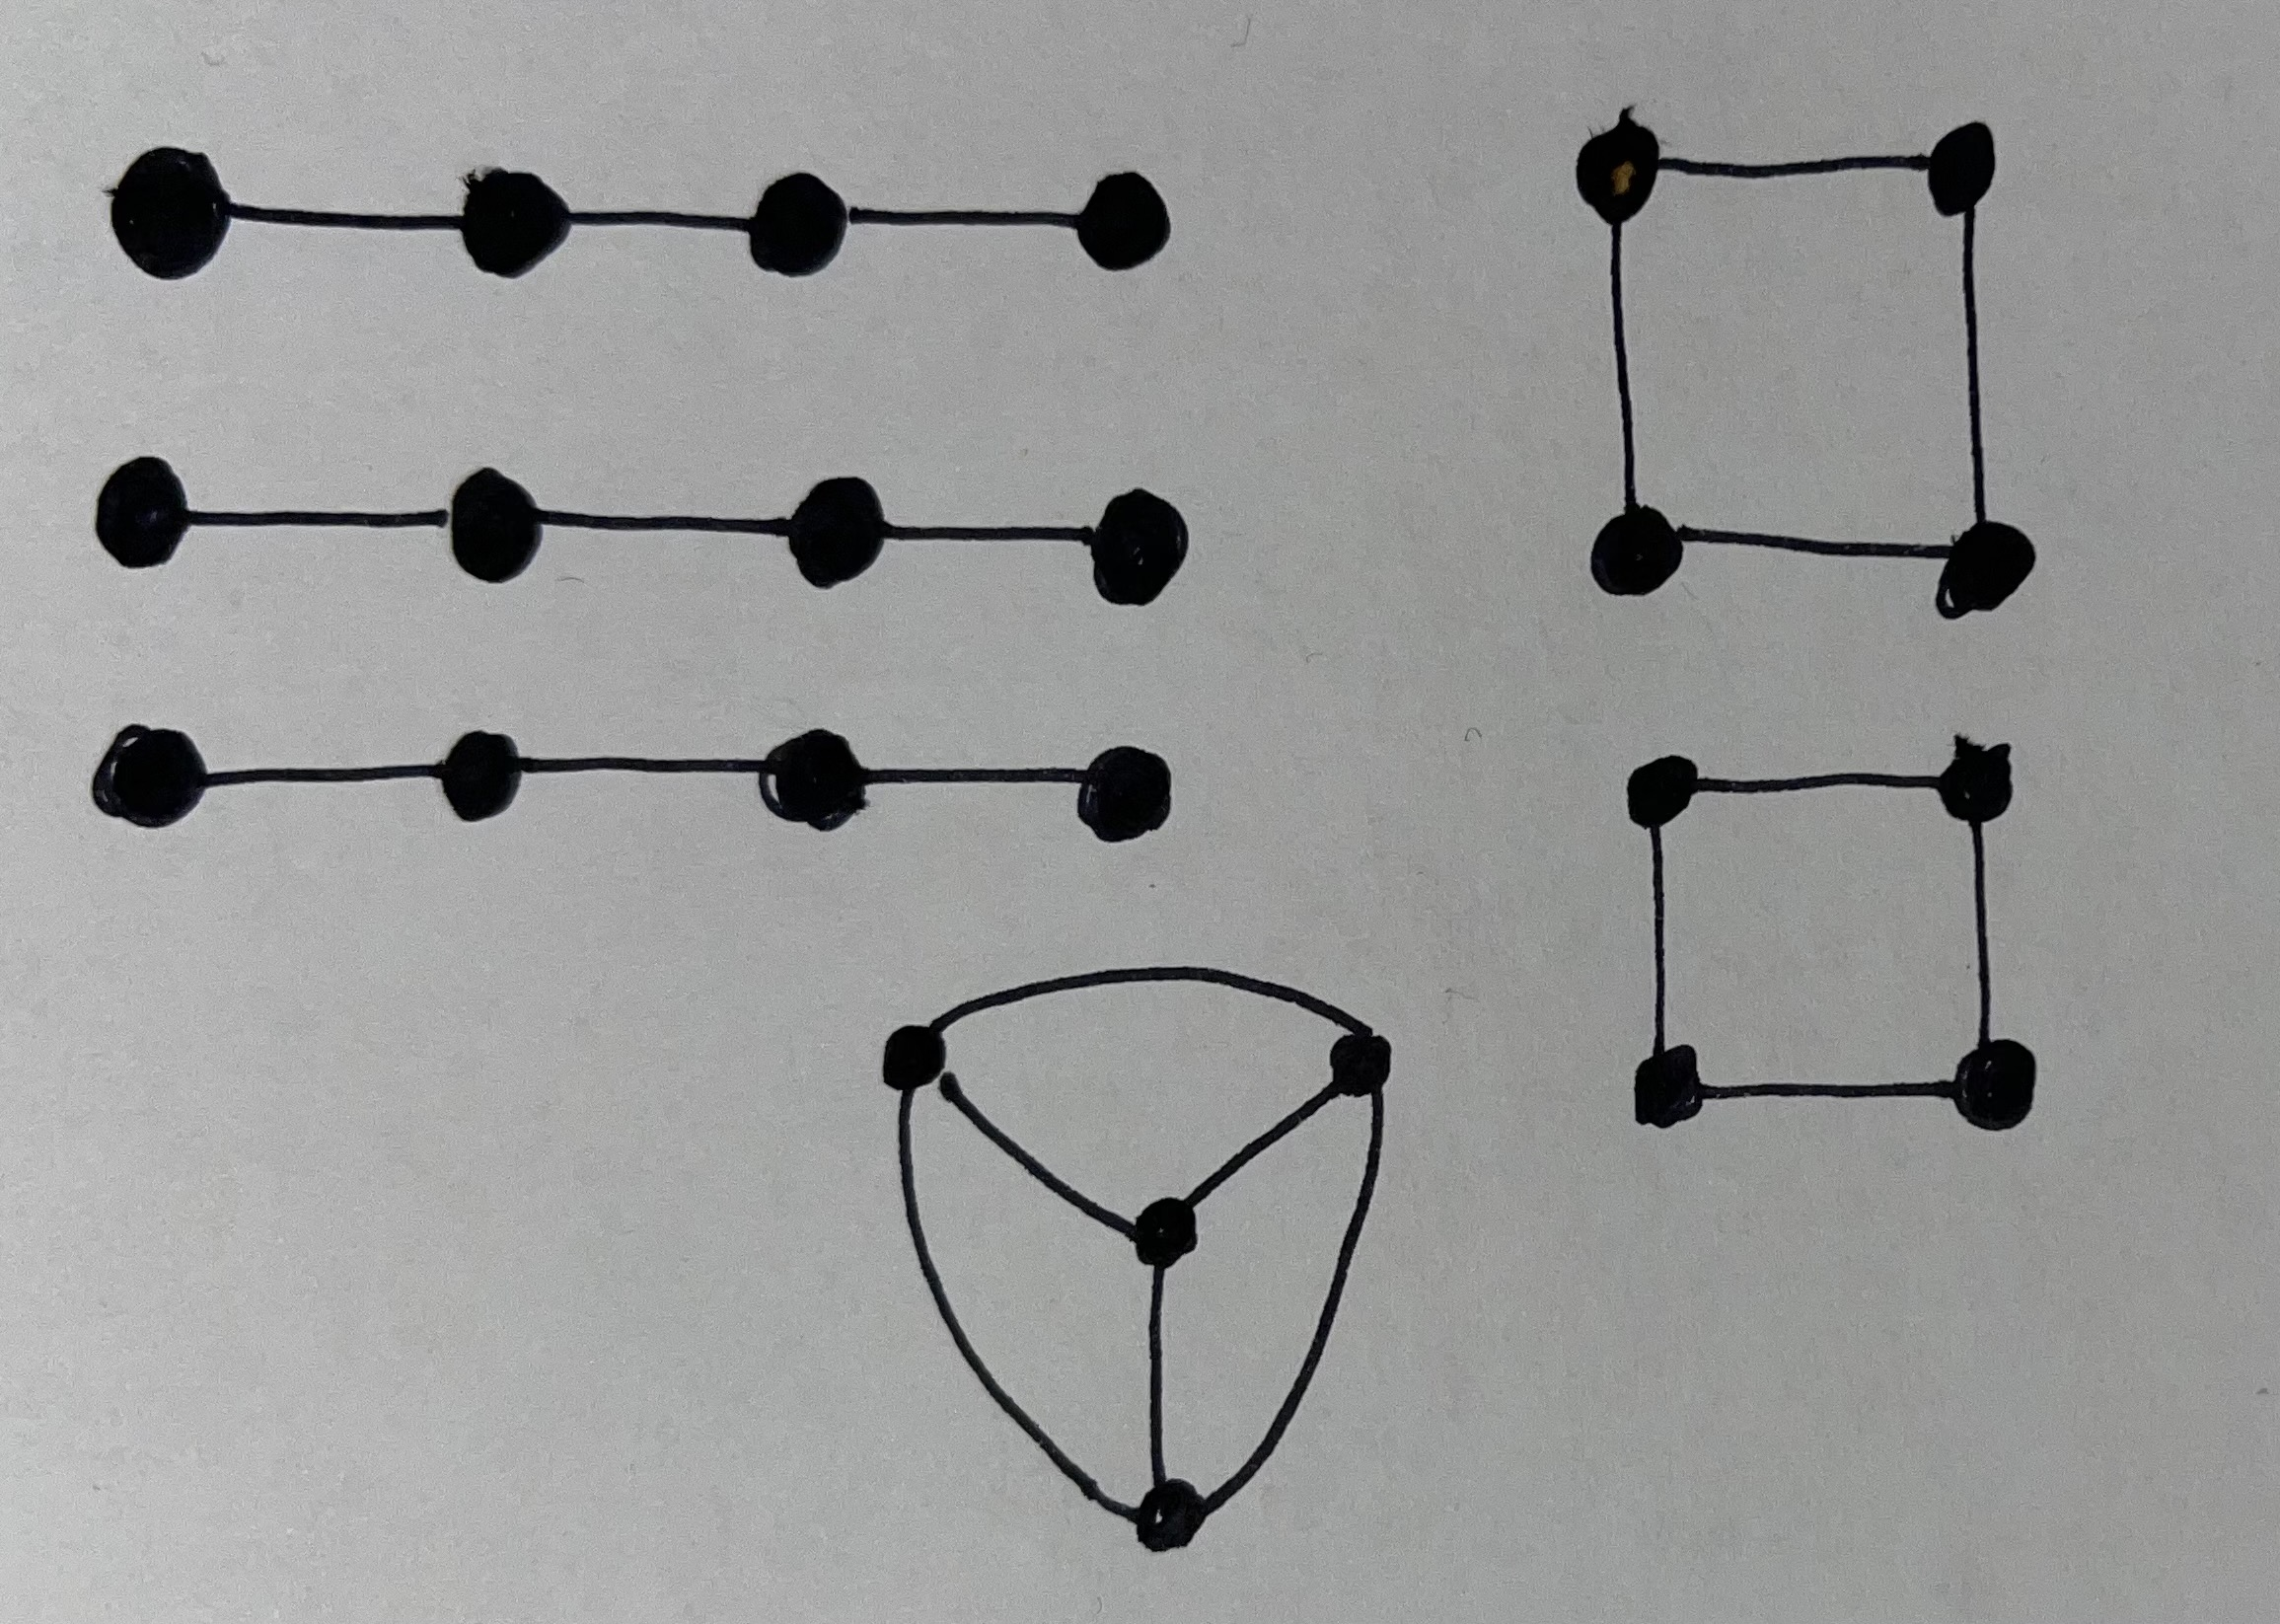
\includegraphics[scale=.05]{HW2-graph1.JPG}
\end{center}

\bigskip
\noindent{\bf 1.22}

\noindent{\bf Proposition}: Let $G$ be a disconnected graph. If $u,v \in V(\overline{G})$, then $d_{\overline{G}}(u,v) = 1$ or $d_{\overline{G}}(u,v) = 2$.
\begin{proof}
Let $G$ be a disconnected graph.
Then, by Theorem 1.11, $\overline{G}$ is connected.
Let $u,v$ be distinct vertices in $\overline G$.
Suppose $uv \notin E(G)$.
Then, by definition of $\overline{G}$, $uv \in E(\overline{G})$.
Thus, $(u,v)$ is a $u-v$ path of length 1 in $\overline G$, so $d_{\overline{G}}(u,v) = 1$.
Now, suppose $uv \in E(G)$.
Then, by the definition of $\overline{G}$, $uv \notin E({\overline{G}})$.
Since $u$ and $v$ are adjacent in $G$, they are in the same component of $G$.
Since $G$ is disconnected, there exists a vertex $w$ in $G$ that is in a different component of from $u$ and $v$.
Thus, $uw \notin E(G)$, and $vw \notin E(G)$.
Therefore, $uw, vw \in E(\overline G)$.
Observe that $(u, w, v)$ is a $u-v$ path of length $2$ in $\overline G$.
Thus, since $uv \notin E(\overline G)$, $d_{\overline{G}}(u,v) = 2$.
Thus, each pair of distinct vertices in $\overline G$ is of distance either 1 or 2 apart.
\end{proof}

\bigskip
\noindent{\bf 1.24}

    By Theorem 1.12, $G_1$ is bipartite.

    \begin{center}
    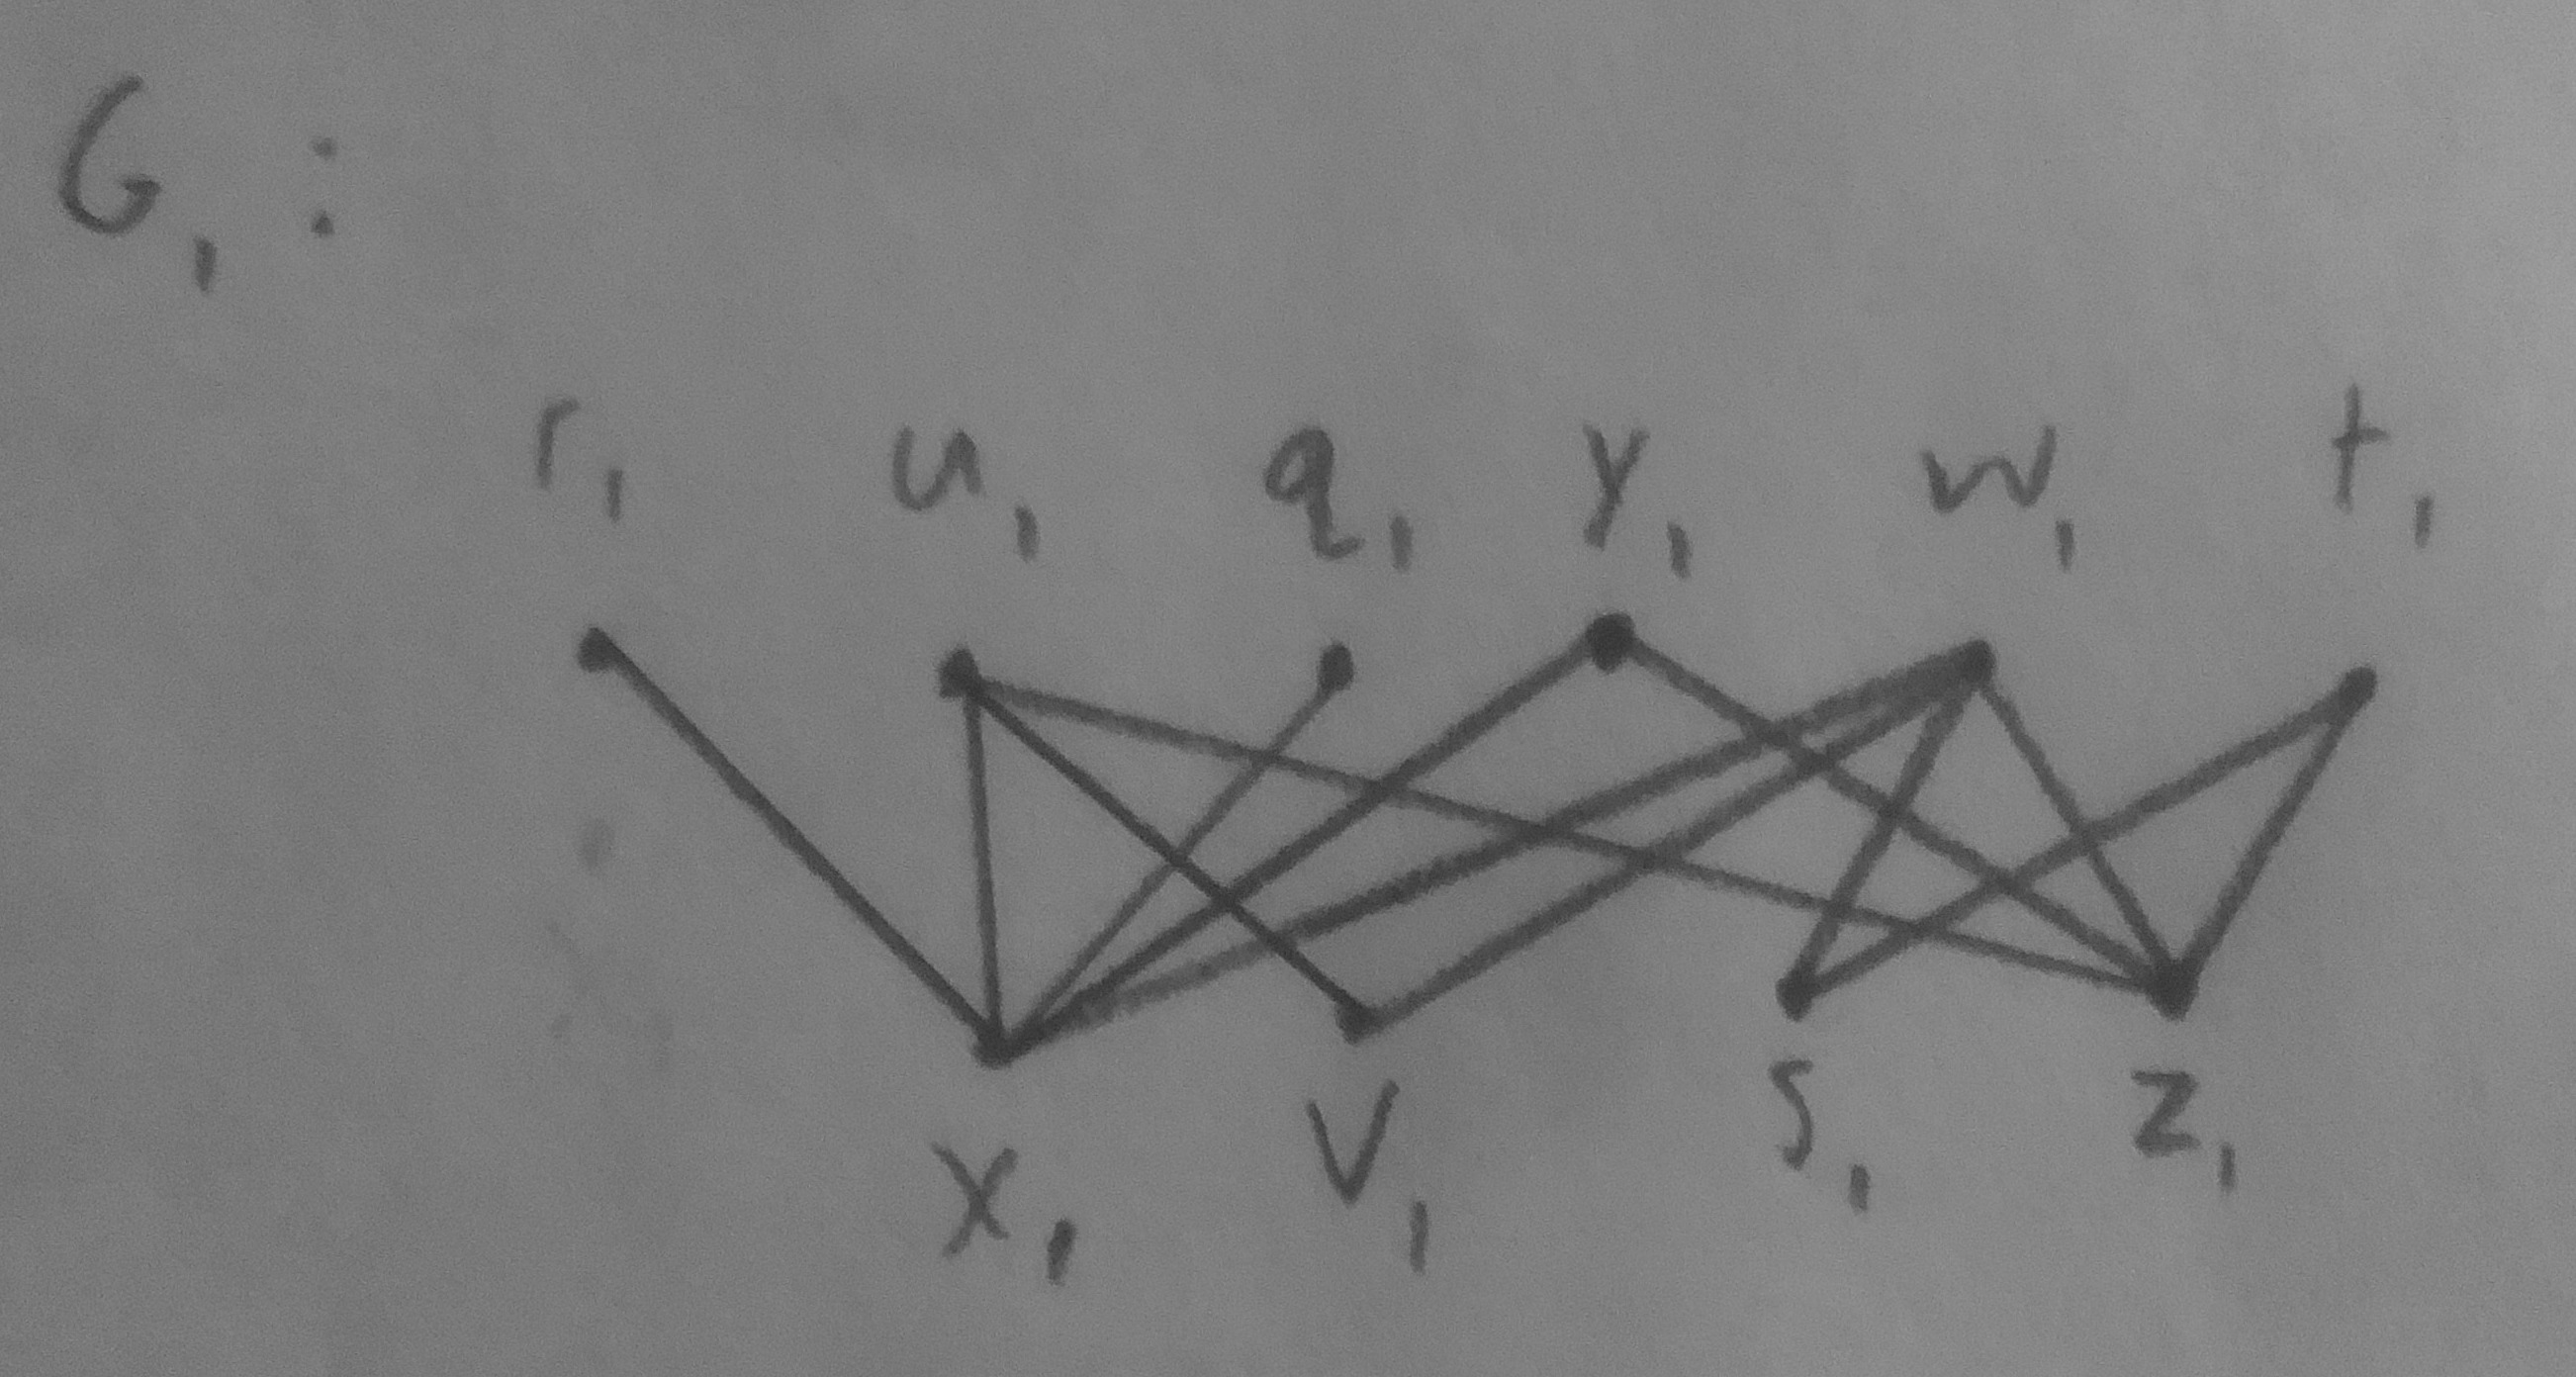
\includegraphics[scale=.1]{graph.jpg}
    \end{center}

    $G_2$ has an odd cycle: $(x_2, r_2, w_2, z_2, y_2, x_2)$. Thus, by Theorem 1.12, $G_2$ is not bipartite.

\end{document}